% Options for packages loaded elsewhere
\PassOptionsToPackage{unicode}{hyperref}
\PassOptionsToPackage{hyphens}{url}
%
\documentclass[
  11pt,
]{article}
\usepackage{amsmath,amssymb}
\usepackage{lmodern}
\usepackage{iftex}
\ifPDFTeX
  \usepackage[T1]{fontenc}
  \usepackage[utf8]{inputenc}
  \usepackage{textcomp} % provide euro and other symbols
\else % if luatex or xetex
  \usepackage{unicode-math}
  \defaultfontfeatures{Scale=MatchLowercase}
  \defaultfontfeatures[\rmfamily]{Ligatures=TeX,Scale=1}
\fi
% Use upquote if available, for straight quotes in verbatim environments
\IfFileExists{upquote.sty}{\usepackage{upquote}}{}
\IfFileExists{microtype.sty}{% use microtype if available
  \usepackage[]{microtype}
  \UseMicrotypeSet[protrusion]{basicmath} % disable protrusion for tt fonts
}{}
\makeatletter
\@ifundefined{KOMAClassName}{% if non-KOMA class
  \IfFileExists{parskip.sty}{%
    \usepackage{parskip}
  }{% else
    \setlength{\parindent}{0pt}
    \setlength{\parskip}{6pt plus 2pt minus 1pt}}
}{% if KOMA class
  \KOMAoptions{parskip=half}}
\makeatother
\usepackage{xcolor}
\usepackage[margin=1in]{geometry}
\usepackage{graphicx}
\makeatletter
\def\maxwidth{\ifdim\Gin@nat@width>\linewidth\linewidth\else\Gin@nat@width\fi}
\def\maxheight{\ifdim\Gin@nat@height>\textheight\textheight\else\Gin@nat@height\fi}
\makeatother
% Scale images if necessary, so that they will not overflow the page
% margins by default, and it is still possible to overwrite the defaults
% using explicit options in \includegraphics[width, height, ...]{}
\setkeys{Gin}{width=\maxwidth,height=\maxheight,keepaspectratio}
% Set default figure placement to htbp
\makeatletter
\def\fps@figure{htbp}
\makeatother
\setlength{\emergencystretch}{3em} % prevent overfull lines
\providecommand{\tightlist}{%
  \setlength{\itemsep}{0pt}\setlength{\parskip}{0pt}}
\setcounter{secnumdepth}{-\maxdimen} % remove section numbering
\newlength{\cslhangindent}
\setlength{\cslhangindent}{1.5em}
\newlength{\csllabelwidth}
\setlength{\csllabelwidth}{3em}
\newlength{\cslentryspacingunit} % times entry-spacing
\setlength{\cslentryspacingunit}{\parskip}
\newenvironment{CSLReferences}[2] % #1 hanging-ident, #2 entry spacing
 {% don't indent paragraphs
  \setlength{\parindent}{0pt}
  % turn on hanging indent if param 1 is 1
  \ifodd #1
  \let\oldpar\par
  \def\par{\hangindent=\cslhangindent\oldpar}
  \fi
  % set entry spacing
  \setlength{\parskip}{#2\cslentryspacingunit}
 }%
 {}
\usepackage{calc}
\newcommand{\CSLBlock}[1]{#1\hfill\break}
\newcommand{\CSLLeftMargin}[1]{\parbox[t]{\csllabelwidth}{#1}}
\newcommand{\CSLRightInline}[1]{\parbox[t]{\linewidth - \csllabelwidth}{#1}\break}
\newcommand{\CSLIndent}[1]{\hspace{\cslhangindent}#1}
\usepackage{setspace}\doublespacing
\usepackage{lineno}\linenumbers
\usepackage{booktabs}
\usepackage{longtable}
\usepackage{array}
\usepackage{multirow}
\usepackage{wrapfig}
\usepackage{float}
\usepackage{colortbl}
\usepackage{pdflscape}
\usepackage{tabu}
\usepackage{threeparttable}
\usepackage{threeparttablex}
\usepackage[normalem]{ulem}
\usepackage{makecell}
\usepackage{xcolor}
\ifLuaTeX
  \usepackage{selnolig}  % disable illegal ligatures
\fi
\IfFileExists{bookmark.sty}{\usepackage{bookmark}}{\usepackage{hyperref}}
\IfFileExists{xurl.sty}{\usepackage{xurl}}{} % add URL line breaks if available
\urlstyle{same} % disable monospaced font for URLs
\hypersetup{
  pdftitle={Evolution along allometric lines of least resistance: Morphological differentiation in Pristurus geckos},
  hidelinks,
  pdfcreator={LaTeX via pandoc}}

\title{Evolution along allometric lines of least resistance:
Morphological differentiation in \emph{Pristurus} geckos}
\author{}
\date{\vspace{-2.5em}}

\begin{document}
\maketitle

\begin{center}
\textbf{H{\'{e}}ctor Tejero-Cicu{\'{e}}ndez$^{1,*}$,  Iris Men{\'{e}}ndez$^{2,3}$, Adri{\'{a}}n Talavera, Gabriel Riaño, Marc Sim{\'{o}}-Riudalbas$^{1}$, Bernat Burriel-Carranza$^{1}$, Salvador Carranza$^{1}$, and Dean C. Adams$^{4}$}
\end{center}

\begin{center}04 November, 2022\end{center}

\(^{1}\)Institute of Evolutionary Biology (CSIC-Universitat Pompeu
Fabra), Passeig Marítim de la Barceloneta 37-49, Barcelona 08003, Spain

\(^{2}\)Departamento de Geodinámica, Estratigrafía y Paleontología,
Facultad de Ciencias Geológicas, Universidad Complutense de Madrid,
C/José Antonio Novais 12, Madrid 28040, Spain

\(^{3}\)Departamento de Cambio Medioambiental, Instituto de Geociencias
(UCM, CSIC), C/Severo Ochoa 7, Madrid 28040, Spain

\(^{4}\)Department of Ecology, Evolution, and Organismal Biology, Iowa
State University, Ames, Iowa, 50010 USA

\(^{*}\)Correspondence: Héctor Tejero-Cicuéndez
\href{mailto:cicuendez93@gmail.com}{\nolinkurl{cicuendez93@gmail.com}}

\hfill\break

\textbf{Keywords}: Phenotypic Evolution, Morphospace, Allometry,
\emph{Pristurus} geckos \hfill\break

\textbf{Short Title}: XXX \hfill\break

\textbf{Author Contributions}: All authors collaboratively developed the
concept and contributed to all portions of this manuscript. HT-C, IM,
and DCA performed the analyses. All authors approve of the final product
and are willingly accountable for any portion of the
content.\hfill\break

\textbf{Conflicts of Interests}: The authors declare no conflicts of
interest.\hfill\break

\textbf{Data Archiving}: Data are available on DRYAD
(\url{doi:10.5061/dryad.xwdbrv1f6} (Tejero-Cicuéndez et al. 2021b)).
R-scripts are available at \textbf{XXX}. \hfill\break

\textbf{Acknowledgments}: We thank XYZPDQ\ldots{} This work was
sponsored in part by XXX (to SC) DCA was funded in part by National
Science Foundation Grant DBI-1902511.

\newpage

\hypertarget{abstract}{%
\section{Abstract}\label{abstract}}

asdf

\newpage

\hypertarget{introduction}{%
\section{Introduction}\label{introduction}}

Understanding how phenotypic diversity evolves, and elucidating the
forces that generate and maintain this diversity, are major goals in
evolutionary biology. Because adaptive evolution is the product of
natural selection, changes in ecological selection pressures are
expected to affect the evolutionary trajectory of phenotypic traits that
facilitate an organism's survival in their habitat. Evolutionary theory
predicts that differing habitats will exert unique ecological selection
pressures on organisms, resulting in associations between ecological and
phenotypic traits. Indeed, species inhabiting differing habitats often
display functional, behavioral, or phenotypic differences, that have
presumably been the result of adaptive diversification in their
respective ecological habitats (Collar et al. 2010; Kaliontzopoulou et
al. 2015; Price et al. 2015; Martinez et al. 2021; Kolmann et al. 2022).
\hfill\break

One possible evolutionary outcome of ecological specialization is that
organisms inhabiting similar environments display common phenotypic
characteristics. When such patterns occur repeatedly (e.g., Losos 1992;
Schluter and McPhail 1992), this convergent evolution is treated as
strong evidence of adaptation. Indeed the ecomorphological paradigm
(sensu Arnold 1983) is predicated, in part, on such cases, which
emphasize the strong association between the phenotypic traits that
organisms display (morphological, behavioral, or physiological), and the
ecological characteristics of their habitat that mediate organismal
performance. In vertebrates, ecomorphological trends have been well
studied in numerous taxonomic groups, and include the emblematic
`ecomorphs' of Caribbean \emph{Anolis} lizards that exploit different
microhabitats (Losos 1992, 2009; Mahler et al. 2013), differential beak
morphology in species of Darwin's finches (Schluter and Grant 1984;
Grant and Grant 2006; Reaney et al. 2020), the recurring phenotypes of
African lake cichlids across ecological regimes (Albertson and Kocher
2001; Urban et al. 2022), and the distinct body forms of freshwater
fishes in benthic and limnetic habitats (Jastrebski and Robinson 2004;
Berner et al. 2008; Stuart et al. 2017) among others. \hfill\break

However, while the patterns of morphological differences in distinct
ecological contexts have been well documented, less-well understood is
how this differentiation has been influenced by trait covariation
asociated with body size differences (i.e., allometry). It has long been
recognized that the interrelationships among traits can exert a strong
influence on how phenotypic evolution proceeds, as trait correlations
influence the degree to which phenotypic variation is exposed to
selection (Wagner and Altenberg 1996). Thus, the integration among
traits can constrain phenotypic change in certain directions, or enhance
variation along other phenotypic axes (Schluter 1996; Wagner and
Altenberg 1996; Wagner and Zhang 2011; Klingenberg and Marugán-Lobón
2013; Goswami et al. 2014, 2016; Felice et al. 2018; Navalón et al.
2020). Further, because nearly all linear traits covary strongly with
overall body size (Jolicoeur 1963; Bookstein 2022), allometric trends
could be considered the quintessential expression of phenotypic
integration. Thus, identifying whether allometric patterns differ across
habitats, and how such patterns of trait covariation affect
ecomorphological trends among species utilizing those habitats, remains
an important question worthy of investigation. \hfill\break

The Afro-Arabian geckos in the genus \emph{Pristurus} afford the
opportunity to elucidate the interdigitating effects of allometry and
habitat specialization on clade-level patterns of phenotypic diversity.
Prior work on this system (Tejero-Cicuéndez et al. 2021a) revealed that
the colonization of ground habitats has been a trigger of morphological
change, specifically reflected in an increase in body size and shape
disparity. Interestingly, some ground-dwelling species are among the
largest of the genus and also show increased relative head sizes and
limb proportions, while some other species with this ecological
specialization have evolved to be among the smallest of the group.
Additionally, among the species exploiting rocky habitats (the most
common ecological feature in \emph{Pristurus}), there are also species
with both considerably large and small body sizes (Tejero-Cicuéndez et
al. 2021a). What remains unexplored, however, is how the evolution of
body shape is related to differences in body size and whether habitat
specialization has an impact in this shape-size relationship.
\hfill\break

In this study, we employed a combination of multivariate morphometric
and phylogenetic comparative analyses to interrogate macroevolutionary
patterns of evolutionary allometry in \emph{Pristurus} geckos of
Afro-Arabia. Using phenotypic, phylogenetic, and ecological data, we
first characterized allometric trends in body form in the group, to
discern the extent to which evolutionary allometric trends across the
phylogeny aligned with habitat-based static allometry for species
occupying distinct ecological regimes. We then examined changes in
allometric trends across the phylogeny, and linked these patterns to
overall phenotypic integration, diversification in morphospace, and
habitat utilization among taxa. Our analyses reveal that patterns of
evolutionary allometry across species align with allometric trends
within habitats, demonstrating that the interplay between ecological
specialization and allometric trajectories in species with disparate
body size may play a determinant role in shaping the phenotypic
evolution and hence in adaptive dynamics in this clade.

\hypertarget{materials-and-methods}{%
\section{Materials and Methods}\label{materials-and-methods}}

\hypertarget{data}{%
\subsection{Data}\label{data}}

We used a combination of phenotypic, phylogenetic, and ecological data
to characterize and evaluate intra- and interspecific allometric trends.
The data utilized here were obtained from our prior work on this system
(Tejero-Cicuéndez et al. 2021a, 2022), and are briefly described here.
First we used a time-dated, molecular phylogeny that included all
members of the genus \emph{Pristurus}, including several currently
undescribed taxa. The tree was estimated in a Bayesian framework, using
five mitochondrial markers, six nuclear markers, and 21 calibration
points (for details see Tejero-Cicuéndez et al. 2022). Next we
categorized each species as belonging to one of three ecological groups
(ground, rock, or tree), based on descriptions of habitat use found in
the literature (see Tejero-Cicuéndez et al. 2021a). Finally, we obtained
a phenotypic data set containing body size (snout-vent length: SVL) and
eight linear measurements (Figure 1) that described overall body form:
trunk length (TrL), head length (HL), head width (HW), head height (HH),
humerus length (Lhu), ulna length (Lun), femur length (Lfe), and tibia
length (Ltb) (Tejero-Cicuéndez et al. 2021a). We restricted our study to
those species represented by nine or more individuals; resulting in a
dataset of 687 individuals from 25 species (invidivuals per species:
\(\mu=27\); min = 9, max = 56). Species in the phenotypic dataset were
then matched to the phylogeny, which was subsequently pruned to arrive
at the final topology. All measurements were log-transformed prior to
statistical analyses. Additional details regarding data collection and
formal descriptions of each linear measurement may be found in the
original sources (see Tejero-Cicuéndez et al. 2021a, 2022). The data are
found on DRYAD: \url{https://doi.org/10.5061/dryad.xwdbrv1f6}
(Tejero-Cicuéndez et al. 2021b).

\hypertarget{statistical-and-comparative-analyses}{%
\subsection{Statistical and Comparative
Analyses}\label{statistical-and-comparative-analyses}}

We conducted a series of analyses to interrogate allometric trends,
patterns of integration, and macroevolutionary changes in allometry,
relative to differentiation in body form. First we characterized
evolutionary allometry in the genus by performing a phylogenetic
multivariate regression of body form on body size (i.e., SVL), using the
species means as data. We then performed an analogous procedure at the
individual level, regressing body form on body size using our entire
dataset. From both the species-level (phylogenetic) and the
individual-level analyses, we obtained the set of regression
coefficients, and calculated the difference in their angular direction
to describe the extent to which patterns of allometry at the individual
level were concordant with evolutionary allometric trends across
species. \hfill\break

Next we used the dataset containing all individuals to determine whether
trends in static allometry differed across habitat groups. This was
accomplished by performing a multivariate analysis of covariance, with
body size (\(SVL\)), \(habitat\), and \(SVL\times habitat\) as model
effects. Significance was evaluated using 999 iterations of a
permutation procedure, where residuals from a reduced model were
randomly permuted in each permutation (RRPP), model statistics were
recalculated, and used to generate empirical null sampling distributions
to evaluate the observed test statistics (following Freedman and Lane
1983; Collyer and Adams 2007; Collyer et al. 2015). We then compared the
multivariate allometric vectors for each habitat group to one another,
and to a vector representing isometry, by calculating pairwise
differences in their angular direction in morphospace, and evaluating
these relative to empirical sampling distributions obtained through RRPP
(Collyer and Adams 2007; Adams and Collyer 2009; Collyer and Adams
2013). Here, residuals were obtained from a common isometry reduced
model, whose `common slope' component described a pattern of
multivariate isometry, and whose intercepts allowed for differences in
least-squares means among groups. Patterns of multivariate allometry
relative to body size were visualized via regression scores (Drake and
Klingenberg 2008) and predicted lines (Adams and Nistri 2010), based on
the coefficients and fitted values from the linear model described
above. \hfill\break

Additionally, because allometry describes the extent to which traits
covary with body size and with each other (i.e., integration), we
conducted an analysis of integration. Here we characterized the extent
of morphological integration in body form for individuals within each
habitat group by summarizing the dispersion of eigenvalues of their
respective trait covariance matrix (sensu Pavlicev et al. 2009). This
measure (\(V_{rel}\)) was subsequently converted to an effect size (a
\(Z\)-score), which quantified the strength of morphological integration
(Conaway and Adams 2022). We then performed a series of two-sample tests
to compare the strength of morphological integration across habitat
groups, following the procedures of Conaway and Adams (2022).
Additionally and for comparison, we repeated these analyses on the set
of size-standardized trait data, found as a set of shape ratios (sensu
Mosimann 1970) where each trait was divided by body size (Supplemental
Information). \hfill\break

To determine the extent to which static and evolutionary allometry were
concordant, we evaluated the directions in morphospace of both the
evolutionary (species-level) and static (habitat-based) allometric
trends. Specifically, we we obtained the set of regression coefficients
from both the phylogenetic multivariate regression and the multivariate
analysis of covariance analyses above, and calculated the differences in
angular direction between the evolutionary trajectory and the static
allometry trend for each habitat group. The observed angles were then
statistically evaluated relative to empirical sampling distributions
obtained through permutation (RRPP), based on the common isometry
reduced model described above. \hfill\break

Next, to discern how allometric trends resulted in the evolution of
distinct body forms, we examined changes in the body shape proportions
across the phylogeny. Here we treated the head dimensions and limb
dimensions separately, as allometric trends could potentially differ
between these body regions due to differential functional or selective
constraints (Kaliontzopoulou et al. 2010). Because both the head and
limb data were multivariate, we first performed a partial least squares
(PLS) analysis (Rohlf and Corti 2000) of the head traits versus SVL, and
the limb traits versus SVL, to describe the direction of maximal
covaration between each body region and size. Then, we measured the mean
residuals of each species to the allometric trend inferred, which show
if head and limbs proportions of species are greater or smaller than
expected for their body size. The species residuals were then mapped on
the phylogeny of \emph{Pristurus} using a Brownian motion model of
evolution, to qualitatively evaluate shifts in head and limbs
proportionality across the phylogeny for the group. Similarly,
within-species patterns of static allometry were visualized by plotting
regressions of PLS scores on SVL for both head and limb traits
separately. \hfill\break

Finally, to relate within-species allometric trends with patterns of
phenotypic diversification in the group we generated a phylomorphospace,
based on the size-standardized species means obtained from a
phylogenetic regression (see Tejero-Cicuéndez et al. 2021a). Here,
phenotypic similarities among species, relative to their phylogenetic
relationships and habitat affiliations, were observed. Additionally,
representative specimens (scaled to unit size) were also visually
compared to aid in describing these trends. A similar phylomorphospace
was constructed for species means not corrected for body size, and the
phenotypic disparity among species means in each habitat was calculated
and subsequently compared (Supplemental Information). All analyses were
conducted in R 4.2.1 (R Core Team 2022), using \texttt{RRPP} version
1.3.1 (Collyer and Adams 2018; Collyer and Adams 2022) and
\texttt{geomorph} 4.0.4 (Baken et al. 2021), and scripts written by the
authors (available at \textbf{XXX}).

\hypertarget{results}{%
\section{Results}\label{results}}

Using phylogenetic regression, we found significant evolutionary
allometry in body form across species (\(N_{sp}=25\); \(F = 217.9\);
\(Z =5.53\); \(P < 0.001\)). Likewise, when allometry in body form was
examined across individuals, a similar pattern was observed
(\(N_{ind}=687\); \(F = 7910.8\); \(Z =9.20\); \(P < 0.001\)). Further,
the vectors of regression coefficients between the two analyses were
highly correlated (\(\rho = 0.94\)) and were oriented in nearly parallel
directions in morphospace (\(\theta = 1.49^\circ\)). This revealed that
the pattern of multivariate allometry across individuals was concordant
with macroevolutionary trends of interspecific allometry among species
of \emph{Pristurus} across the phylogeny. \hfill\break

Our analyses also exposed significant differences in the allometry of
body form among \emph{Pristurus} utilizing distinct habitats (Table 1).
Further, pairwise comparisons of multivariate allometric vectors
revealed that patterns of static allometry in each habitat differed
significantly from isometry, indicating the presence of multivariate
allometry in each (Table 2). Additionally, comparisons identified that
ground-dwelling \emph{Pristurus} displayed the most distinct allometric
trend as compared with \emph{Pristurus} occupying both the rock and tree
habitats (Table 2; Figure 2). Inspection of the regression coefficients
for each trait (Supplemental Information) revealed that allometry in
this group was exemplified by steeper allometric coefficients for all
head and limb traits as compared with rock and tree-dwelling taxa. These
findings implied that larger individuals of ground-dwelling
\emph{Pristurus} species displayed disproportionately larger heads and
limbs, as compared with large individuals in taxa utilizing other
habitat types. Multivariate visualizations of these multivariate
allometric trends (Figure 2) confirmed these statistical findings, and
indicated that the allometric trajectory in ground-dwelling
\emph{Pristurus} was more extreme as compared with either rock or
tree-dwelling \emph{Pristurus}. \hfill\break

Examination of patterns of trait covariation revealed strong levels of
morphological integration within each habitat type (\(Z_{ground}=3.97\);
\(Z_{rock}=3.72\); \(Z_{tree}=2.15\)). Further, two-sample tests
revealed that the strength of morphological integration was
significantly greater in ground-dwelling \emph{Pristurus} than either
those utilizing rock (\(Z_{Groung-Rock}=6.59\); \(P << 0.001\)) or tree
habitats (\(Z_{Groung-Tree}=11.17\); \(P << 0.001\)). \emph{Pristurus}
utilizing tree habitats displayed the lowest levels of integration,
which were also significantly less than in the rock habitat
(\(Z_{Rock-Tree}=7.19\); \(P << 0.001\)). When size was accounted for in
the data, levels of integration dropped considerably, though the overall
pattern and differences among habitat groups remained the same
(Supplemental Information). \hfill\break

Comparisons of evolutionary allometry with static allometry in each
habitat revealed substantial concordance between these allometric
trends. Here, vectors of regression coefficients representing static
allometry within habitat groups were oriented in very similar directions
with the regression vector representing evolutionary allometry, with
small pairwise angles between them
(\(\theta: 2.3^\circ\rightarrow5.9^\circ\)). Subsequent permutation
tests indicated no differences between the static allometry vectors and
the regression vector representing evolutionary allometry, indicating
strong congruence between them (Table 3). Notably, static allometry in
ground-dwelling \emph{Pristurus} was most similar to trends of
evolutionary allometry, displaying the smallest angular difference and
largest effect size. Thus, static and evolutionary allometry trends were
essentially parallel in this group, indicating a direct correspondence
between the two. This result implied that phenotypic evolution across
species aligned closely with directions of allometric variation within
habitat groups at the individual level; namely that larger individuals
and larger ground-dwelling species exhibited disproportionately larger
heads and limbs, while smaller individuals and smaller ground-dwelling
species displayed disproportionately smaller heads and limbs.
\hfill\break

Mapping the residuals of species into the phylogeny showed that large
ground-dwelling species displayed greater head proportions than large
rock-dwelling species, who exhibited smaller heads relative to body size
(Figure 3A). Conversely, the opposite pattern was observed when
comparing small species utilizing these habitats: ground-dwelling
species showed small relative head proportions while rock-dwelling
species displayed generally larger head proportions. In contrast, limb
shape showed more variable patterns. Although all large ground-dwelling
species consistently displayed large relative limb proportions, large
rock-dwelling species were more variable in this trait, with \emph{P.
insignis} exhibiting large and \emph{P. insignoides} small limb
proportions. For small species, shifts in relative limb proportions
seemed more independent of habitat utilization, since there were
differences in limb residuals both within rock- and ground-dwelling
species (Figure 3B). Visual inspection of static allometry trends within
species (Figure 4) largely confirmed these patterns, illustrating that
ground-dwelling species generally displayed steeper allometric patterns
as compared with rock-dwelling species. Overall there was general
concordance across taxa in terms of trends of multivariate allometry,
affirming that the association between evolutionary allometry and
habitat-based static allometry was robust. \hfill\break

Viewing body shape differentiation in \emph{Pristurus} in
phylomorphospace (Figure 5) revealed broad overlap among habitat groups,
though arboreal (tree-dwelling) species were somewhat more separated in
morphospace. Rock-dwelling species occupied a slightly larger region of
morphospace as compared with the other groups, though this pattern was
not statistically significant (Supplemental Information). Intriguingly,
when viewed in relation to body size, large \emph{Pristurus} species
were not localized to a particular region of morphospace, nor were
smaller species. Instead, the largest rock-dwelling species were found
in close proximity to the smallest ground-dwelling species, indicating
that they were similar in overall body shape. Likewise, the smaller
rock-dwelling species were found close to large ground-dwelling species
in morphospace, indicating they displayed similar body shapes as well.
\hfill\break 

Finally, when representative specimens were scaled to a similar body
size (Figure 6), the consequences of differences in allometric trends on
body proportions became apparent. Here, larger ground-dwelling
\emph{Pristurus} species displayed disproportionately larger heads and
limbs as compared with large \emph{Pristurus} species utilizing other
habitat types. Conversely, smaller rock-dwelling \emph{Pristurus}
species were found to have disproportionately larger heads and limbs as
compared with smaller \emph{Pristurus} ground-dwelling species. These
patterns corresponded closely with those identified in morphospace
(Figure 5), where large ground-dwelling species were similar in body
form to small rock-dwelling species, while small ground-dwelling species
were similar in body form to large rock-dwelling species (Figure 6).
Thus, synthesizing the patterns revealed in the phylomorphospace with
those from the other analyses revealed that the same body shape could be
obtained in different ways, as determined by subtle differences in
allometric slope across habitats, combined with body size differences.
As such, species with similar body shapes displayed differing overall
size, were found in distinct habitats, and exhibited different
allometric trends. \hfill\break

\hypertarget{discussion}{%
\section{Discussion}\label{discussion}}

The relationship between ecologically-relevant phenotypic traits and the
organisms' environment is a central paradigm in evolutionary biology. In
this context, disentangling the causes of phenotypic differentiation is
essential to understand how natural selection operates. In this study,
we evaluated the role of potential drivers of body shape differentiation
in the geckos of the genus \emph{Pristurus}. To this end, we
investigated the interplay of ecological specialization, phenotypic
integration and allometric trends to decipher how they have shaped
patterns of morphological evolution in this radiation of Afro-Arabian
geckos. Our results show that allometric trends and integration patterns
are different across habitats, with ground-dwelling species having the
steepest multivariate allometric slope and also the strongest
morphological integration. These patterns are also different across body
parts, with decoupled trends between head and limb proportions.
Additionally, we found that changes in static allometric trends are not
restricted to specific regions of the phylogeny, but rather they show
multiple independent increases and decreases following common dynamics
within habitat groups. These findings have several important
implications for how allometric trends relate to patterns of phenotypic
diversity generally, and the evolution of phenotypic diversification in
\emph{Pristurus} in particular. \hfill\break

\textbf{remove the different head vs.~limb? Mention below but not a main
result}

\textbf{Also, bring in static vs.~evol. allometry here}

First, \ldots{}

\begin{itemize}
\tightlist
\item
  result 1: allometry; overall trend among species nearly identical to
  that among individuals.
\end{itemize}

Patterns of multivariate allometry in body form calculated from
individuals were found to be nearly identical to those calculated from
per-species means in Pristurus geckos. Specifically, the vectors of
regression coefficients of the two analyses are virtually parallel
(\(\theta = 1.49^\circ\)), indicating that the evolutionary allometry is
not substantially different whether measured with individual
measurements or with species means in this genus.

\textbf{??We also explored patterns of static allometry to compare them
among species and with general trends of evolutionary allometry.}

\begin{itemize}
\tightlist
\item
  result 2: Allometry differs among habitat groups: `steeper' allometry
  in Ground-dwelling (implication: disproportionately larger heads and
  longer limbs in species at larger body sizes).
\end{itemize}

When we compared multivariate allometric slopes of species occupying
different habitats, we found that, while rock-dwelling and arboreal
species do not significantly differ from the isometric trend,
ground-dwelling species have a steeper slope which is statistically
different from isometry. This means that large ground-dwelling
\emph{Pristurus} present disproportionately larger heads and longer
limbs relative to other large species, while small species in the ground
have disproportionately smaller heads and shorter limbs (\textbf{Figure
residuals traitgrams}). This is consistent with previous results on the
morphological evolution of \emph{Pristurus} (Tejero-Cicuéndez et
al.~2021), where large ground species were indeed found to have also
disproportionately large heads and long limbs. This suggests that the
segregation in body size and shape through differential allometric
relationships across habitats responds to adaptive dynamics concerning
the colonization of ground habitats, and perhaps with a particular
interest of hard ground environments inhabited by the largest
ground-dwelling species (including the largest of the genus, \emph{P.
carteri}), which has already been suggested to be the main driver of the
morphological evolution in this genus (Tejero-Cicuéndez et al.~2021).
This points toward the existence of a specialized form of
\emph{Pristurus} geckos adapted to hard grounds (e.g., \textbf{some
definition of hard ground vs.~soft grounds??}), illustrating the
ecomorphological relationships in the genus with a rather conspicuous
`ecomorph' (see Figure X for an example of the hard-ground ecomorph,
\emph{P. carteri}).

\begin{itemize}
\tightlist
\item
  result 3: relationship between evolutionary and static allometry,
  evolution of static allometry mapped in the phylogeny\ldots{}
\end{itemize}

There is no general consensus about the relationship between the three
types of allometry: ontogenetic (allometry during the development),
static (allometry among individuals at the same developmental stage),
and evolutionary (allometry across populations or species). This, in
turn, is reflected in the broadly ambiguous interpretation of allometric
patterns in the literature, with an often uncertain distinction between
allometry as an evolutionary constraint and allometry as functional
optimization resulting from natural selection (Pélabon et al.~2014, Voje
et al.~2014). Even though testing these alternative hypotheses is beyond
the scope of this work, our results do suggest that static and
evolutionary allometry are very similar in \emph{Pristurus} geckos,
which could be explained by low evolvability of allometry, but also by
the effect of relatively homogeneous selective pressures at different
scales. Further analyses, for instance including a broader phylogenetic
context and developmental assessments, are needed to illuminate the
relationships between different levels of allometric trends.
\textbf{EXTEND THIS}

\begin{itemize}
\tightlist
\item
  result 4: Morphological integration differs among habitat groups.
  Strongest in ground-dwelling; weakest in tree-dwelling. SOME MEANING
  (combined with allometric trend implies that patterns of trait
  covariation are more constrained within ground-dwelling\ldots. Thus,
  differences in body form are most likely found along this primary
  axis\ldots{} (harken to Schluter evolution along lines of least
  resistance)

  \begin{itemize}
  \tightlist
  \item
    Additionally, rank-order of magnitude of integration across habitat
    groups corresponds with the range of body sizes in each:
    ground-dwelling display the largest size-range, while tree-dwelling
    the least (Supp. Information). On the one hand this matches the
    expectation that much of the integration observed in
    \emph{Pristurus} is the result of allometric trends\ldots. And the
    fact that levels of integration drop so precipitously when data are
    size-standardized are in accord with this interpretation.
    Nevertheless, when size is accounted for, the rank-order of
    magnitudes of integration remain the same, implying that
    ground-dwelling \emph{Pristurus} are still relatively constrained in
    patterns of trait covariation as compared with the other two
    groups.\\
  \item
    This notion was further supported when viewing the phylomorphospace
    of the species means not adjusted for size (SI). Here (and not
    surprisingly), PC1 is dominated by size, with small species at one
    end and larger species at the other. More importantly however, is
    that the disparity among species utilizing different habitats
    differed significantly in this space. Here, ground-dwelling
    displayed significantly greater phenotypic disparity than did the
    other groups (SI).
  \end{itemize}
\end{itemize}

Similarly, when analyzing patterns of morphological integration, we
found important differences among habitat groups: ground-dwelling
species present the strongest integration, which in turn is weakest in
arboreal species. Morphological integration occurs when different body
parts coevolve, and has been suggested as an evolutionary constraint,
since it restricts the specific lines along which integrated structures
are allowed to vary (\textbf{REF}). Weaker integration levels (i.e.,
modularity), on the contrary, might facilitate morphological evolution
by allowing a less constrained exploration of the morphospace
(\textbf{REF}). However, integration might also be interpreted as a
potential driver of morphological change, since it may provide a
phenotypic pathway through adaptive lines of least resistance that
enable rapid evolutionary processes (Navalón et al. 2020). In this
context, our results on allometry and integration suggest that patterns
of trait covariation are more constrained in ground-dwelling species,
such that their differences in body form are most likely found along
this primary axis. The fact that ground species in \emph{Pristurus} have
been found to have the widest phenotypic disparity and highest rates of
morphological evolution (Tejero-Cicuéndez et al.~2021) is consistent
with the idea that integration patterns are acting to facilitate
morphological evolution along lines of least resistance.

\begin{itemize}
\item
  result 5: morphospace: Thus there was a reciprocal relationship
  between body shape and body size across ground-dwelling and
  rock-dwelling species. SOMEHOW TIE THIS TO integration (DCA pondering
  this one)
\item
  one interesting\ldots{} head vs.~(correlation of head vs.~limb slopes:
  0.42. Pretty low. Implies some sort of differential something here,
  resulting in distinct allometric patterns for these two body regions.
  SImilar to Antigoni's work (and refs therein). IMPLICATION: tie this
  into integration/modularity. Less integrated across the whole
  organism, and more modular\ldots{} Future studies should examine this.
\end{itemize}

Another insightful result is the low correlation between head and limbs
in their allometric slopes, which implies different evolutionary
trajectories for these two body regions. This is likely to happen when
different parts of an organism are subjected to different functional
pressures (e.g., head evolution might be mainly influenced by diet while
limb evolution might respond more tightly to the substrate used by the
species), resulting in a decoupling of their respective morphological
change. Ultimately, the combination of selective pressures upon which
organisms evolve may lead to differential levels of integration across
different body parts, with certain structures coevolving in a similar
(i.e., integrated) manner and others in a segregated (i.e., modular)
way. This, in turn, may have fundamental implications for the extent of
morphological diversification within clades, and can be key to describe
the phenotypic divergence observed across the tree of life. Future and
more in-depth studies on the evolution of different body parts in
\emph{Pristurus} and other lizards, including for instance finer
phenotypic data and comprehensive ecological information, may allow for
discerning the functional drivers of head and limb evolution.

\begin{itemize}
\tightlist
\item
  In conclusion\ldots{} -Synthesizing these patterns together \ldots{}
  (summarize: steeper allometry, higher integration, greater disparity
  in body size and body form all in ground-dwelling species). TOgether
  the patterns uncovered in our study imply that phenotypic
  diversification among ground-dwelling \emph{Pristurus} follows tightly
  along its allometric trajectory, as evidenced by the higher disparity
  and stronger morphological integration\ldots. some reference back to
  Goswami `fly in a tube' paper. Thus, \emph{Pristurus body forms appear
  to diversify along }allometric* lines of least resistance\ldots.
  (Schluter ref again)
\end{itemize}

\newpage

\hypertarget{references}{%
\section*{References}\label{references}}
\addcontentsline{toc}{section}{References}

\setlength{\parindent}{-0.25in} \setlength{\leftskip}{0.25in}
\setlength{\parskip}{8pt} \noindent

\hypertarget{refs}{}
\begin{CSLReferences}{1}{0}
\leavevmode\vadjust pre{\hypertarget{ref-AdamsCollyer2009}{}}%
Adams, D. C., and M. L. Collyer. 2009. A general framework for the
analysis of phenotypic trajectories in evolutionary studies. Evolution
63:1143--1154.

\leavevmode\vadjust pre{\hypertarget{ref-AdamsNistri2010}{}}%
Adams, D. C., and A. Nistri. 2010. Ontogenetic convergence and evolution
of foot morphology in european cave salamanders (family:
plethodontidae). BMC Evolutionary Biology 10:1--10. BioMed Central.

\leavevmode\vadjust pre{\hypertarget{ref-Albertson2001}{}}%
Albertson, R. C., and T. D. Kocher. 2001. Assessing morphological
differences in an adaptive trait: A landmark-based morphometric
approach. Journal of Experimental Zoology 289:385--403.

\leavevmode\vadjust pre{\hypertarget{ref-Arnold1983}{}}%
Arnold, S. J. 1983. Morphology, performance, fitness. American Zoologist
23:347--361.

\leavevmode\vadjust pre{\hypertarget{ref-Baken2021}{}}%
Baken, E. K., M. L. Collyer, A. Kaliontzopoulou, and D. C. Adams. 2021.
Geomorph 4.0 and gmShiny: Enhanced analytics and a new graphical
interface for a comprehensive morphometric experience. Methods in
Ecology and Evolution 12:2355--2363.

\leavevmode\vadjust pre{\hypertarget{ref-BERNER2008}{}}%
Berner, D., D. C. Adams, A.-C. Grandchamp, and A. P. Hendry. 2008.
Natural selection drives patterns of lake-stream divergence in
stickleback foraging morphology. Journal of Evolutionary Biology
21:1653--1665.

\leavevmode\vadjust pre{\hypertarget{ref-Bookstein2022}{}}%
Bookstein, F. L. 2022. Dimensions of morphological integration.
Evolutionary Biology 49:342--372.

\leavevmode\vadjust pre{\hypertarget{ref-COLLAR2010}{}}%
Collar, D. C., J. A. Schulte, B. C. O'Meara, and J. B. Losos. 2010.
Habitat use affects morphological diversification in dragon lizards.
Journal of Evolutionary Biology 23:1033--1049.

\leavevmode\vadjust pre{\hypertarget{ref-CollyerAdams2007}{}}%
Collyer, M. L., and D. C. Adams. 2007. Analysis of two-state
multivariate phenotypic change in ecological studies. Ecology
88:683--692.

\leavevmode\vadjust pre{\hypertarget{ref-CollyerAdams2013}{}}%
Collyer, M. L., and D. C. Adams. 2013. Phenotypic trajectory analysis:
Comparison of shape change patterns in evolution and ecology. Hystrix
24:75--83.

\leavevmode\vadjust pre{\hypertarget{ref-RRPP}{}}%
Collyer, M. L., and D. C. Adams. 2022.
\href{https://CRAN.R-project.org/package=RRPP}{R: RRPP: Linear model
evaluation with randomized residuals in a permutation procedure. Vsn.
1.3.1}. R Foundation for Statistical Computing, Vienna, Austria.

\leavevmode\vadjust pre{\hypertarget{ref-CollyerAdams2018}{}}%
Collyer, M. L., and D. C. Adams. 2018. RRPP: An r package for fitting
linear models to high-dimensional data using residual randomization.
Methods in Ecology and Evolution 9:1772--1779.

\leavevmode\vadjust pre{\hypertarget{ref-Collyer_et_al2015}{}}%
Collyer, M. L., D. J. Sekora, and D. C. Adams. 2015. A method for
analysis of phenotypic change for phenotypes described by
high-dimensional data. Heredity 115:357--365.

\leavevmode\vadjust pre{\hypertarget{ref-ConawayAdams2022}{}}%
Conaway, M. A., and D. C. Adams. 2022.
\href{https://doi.org/10.1111/evo.14595}{An effect size for comparing
the strength of morphological integration across studies}. Evolution
76:(In Press).

\leavevmode\vadjust pre{\hypertarget{ref-DrakeKlingenberg2008}{}}%
Drake, A. G., and C. P. Klingenberg. 2008.
\href{https://doi.org/10.1098/rspb.2007.1169}{The pace of morphological
change: Historical transformation of skull shape in st bernard dogs}.
Proceedings of the Royal Society B: Biological Sciences 275:71--76.

\leavevmode\vadjust pre{\hypertarget{ref-Felice2018}{}}%
Felice, R. N., M. Randau, and A. Goswami. 2018. A fly in a tube:
Macroevolutionary expectations for integrated phenotypes. Evolution
72:2580--2594.

\leavevmode\vadjust pre{\hypertarget{ref-Freedman1983}{}}%
Freedman, D., and D. Lane. 1983. A nonstochastic interpretation of
reported significance levels. Journal of Business {\&} Economic
Statistics 1:292--298.

\leavevmode\vadjust pre{\hypertarget{ref-Goswami2016}{}}%
Goswami, A., M. Randau, P. D. Polly, V. Weisbecker, C. Verity Bennett,
L. Hautier, and M. R. Sánchez-Villagra. 2016.
\href{https://doi.org/10.1093/icb/icw039}{Do developmental constraints
and high integration limit the evolution of the marsupial oral
apparatus?} Integrative and Comparative Biology 56:404--415.

\leavevmode\vadjust pre{\hypertarget{ref-Goswami2014}{}}%
Goswami, A., J. B. Smaers, C. Soligo, and P. D. Polly. 2014.
\href{https://doi.org/10.1098/rstb.2013.0254}{The macroevolutionary
consequences of phenotypic integration: From development to deep time}.
Philosophical Transactions of the Royal Society B: Biological Sciences
369:20130254.

\leavevmode\vadjust pre{\hypertarget{ref-Grant2006}{}}%
Grant, P. R., and B. R. Grant. 2006. Evolution of character displacement
in darwin's finches. Science 313:224--226.

\leavevmode\vadjust pre{\hypertarget{ref-Jastrebski2004}{}}%
Jastrebski, C. J., and B. W. Robinson. 2004. Natural selection and the
evolution of replicated trophic polymorphisms in pumpkinseed sunfish
(\emph{{L}epomis gibbosus}). Evolutionary Ecology Research 6:285--305.

\leavevmode\vadjust pre{\hypertarget{ref-Jolicoeur1963}{}}%
Jolicoeur, P. 1963. The multivariate generalization of the allometry
equation. Biometrics 19:497--499.

\leavevmode\vadjust pre{\hypertarget{ref-Kaliontzopoulou2015}{}}%
Kaliontzopoulou, A., M. A. Carretero, and D. C. Adams. 2015.
Ecomorphological variation in male and female wall lizards and the
macroevolution of sexual dimorphism in relation to habitat use. Journal
of Evolutionary Biology 28:80--94.

\leavevmode\vadjust pre{\hypertarget{ref-KALIONTZOPOULOU2010}{}}%
Kaliontzopoulou, A., M. A. Carretero, and G. A. Llorente. 2010.
Intraspecific ecomorphological variation: Linear and geometric
morphometrics reveal habitat-related patterns within \emph{{P}odarcis
bocagei} wall lizards. Journal of Evolutionary Biology 23:1234--1244.

\leavevmode\vadjust pre{\hypertarget{ref-Klingenberg2013}{}}%
Klingenberg, C. P., and J. Marugán-Lobón. 2013. Evolutionary covariation
in geometric morphometric data: Analyzing integration, modularity, and
allometry in a phylogenetic context. Systematic Biology 62:591--610.

\leavevmode\vadjust pre{\hypertarget{ref-Kolmann2022}{}}%
Kolmann, M. A., F. P. L. Marques, J. C. Weaver, M. N. Dean, J. P.
Fontenelle, and N. R. Lovejoy. 2022. Ecological and phenotypic
diversification after a continental invasion in neotropical freshwater
stingrays. Integrative and Comparative Biology 62:424--440.

\leavevmode\vadjust pre{\hypertarget{ref-Losos2009}{}}%
Losos, J. B. 2009. Lizards in an evolutionary tree: Ecology and adaptive
radiation of anoles. University of California Press.

\leavevmode\vadjust pre{\hypertarget{ref-Losos1992}{}}%
Losos, J. B. 1992. The evolution of convergent structure in {C}aribbean
\emph{{A}nolis} communities. Systematic Biology 41:403--420.

\leavevmode\vadjust pre{\hypertarget{ref-Mahler2013}{}}%
Mahler, D. L., T. Ingram, L. J. Revell, and J. B. Losos. 2013.
Exceptional convergence on the macroevolutionary landscape in island
lizard radiations. Science 341:292--295.

\leavevmode\vadjust pre{\hypertarget{ref-Martinez2021}{}}%
Martinez, C. M., S. T. Friedman, K. A. Corn, O. Larouche, S. A. Price,
and P. C. Wainwright. 2021. The deep sea is a hot spot of fish body
shape evolution. Ecology Letters 24:1788--1799.

\leavevmode\vadjust pre{\hypertarget{ref-Mosimann1970}{}}%
Mosimann, J. E. 1970. Size allometry: Size and shape variables with
characterizations of the lognormal and generalized gamma distributions.
Journal of the American Statistical Association 65:930--945.

\leavevmode\vadjust pre{\hypertarget{ref-Navalon2020}{}}%
Navalón, G., J. Marugán-Lobón, J. A. Bright, C. R. Cooney, and E. J.
Rayfield. 2020. The consequences of craniofacial integration for the
adaptive radiations of darwin's finches and hawaiian honeycreepers.
Nature Ecology \& Evolution 4:270--278. Nature Publishing Group.

\leavevmode\vadjust pre{\hypertarget{ref-Pavlicev2009}{}}%
Pavlicev, M., J. M. Cheverud, and G. P. Wagner. 2009.
\href{https://doi.org/10.1007/s11692-008-9042-7}{Measuring morphological
integration using eigenvalue variance}. Evolutionary Biology
36:157--170.

\leavevmode\vadjust pre{\hypertarget{ref-Price2015}{}}%
Price, S. A., S. T. Friedman, and P. C. Wainwright. 2015. How predation
shaped fish: The impact of fin spines on body form evolution across
teleosts. Proceedings of the Royal Society B: Biological Sciences
282:20151428.

\leavevmode\vadjust pre{\hypertarget{ref-RCT}{}}%
R Core Team. 2022. \href{https://www.R-project.org/}{R: A language and
environment for statistical computing. Version 4.2.1}. R Foundation for
Statistical Computing, Vienna, Austria.

\leavevmode\vadjust pre{\hypertarget{ref-Reaney2020}{}}%
Reaney, A. M., Y. Bouchenak-Khelladi, J. A. Tobias, and A. Abzhanov.
2020. Ecological and morphological determinants of evolutionary
diversification in darwin{\textquotesingle}s finches and their
relatives. Ecology and Evolution 10:14020--14032.

\leavevmode\vadjust pre{\hypertarget{ref-Rohlf2000}{}}%
Rohlf, F. J., and M. Corti. 2000. Use of two-block partial least-squares
to study covariation in shape. Systematic Biology 49:740--753.

\leavevmode\vadjust pre{\hypertarget{ref-Schluter1996}{}}%
Schluter, D. 1996. Adaptive radiation along genetic lines of least
resistance. Evolution 50:1766--1774.

\leavevmode\vadjust pre{\hypertarget{ref-Schluter1984}{}}%
Schluter, D., and P. R. Grant. 1984. Determinants of morphological
patterns in communities of darwin{\textquotesingle}s finches. The
American Naturalist 123:175--196.

\leavevmode\vadjust pre{\hypertarget{ref-Schluter1992}{}}%
Schluter, D., and J. D. McPhail. 1992. Ecological character displacement
and speciation in sticklebacks. The American Naturalist 140:85--108.

\leavevmode\vadjust pre{\hypertarget{ref-Stuart2017}{}}%
Stuart, Y. E., T. Veen, J. N. Weber, D. Hanson, M. Ravinet, B. K.
Lohman, C. J. Thompson, T. Tasneem, A. Doggett, R. Izen, N. Ahmed, R. D.
H. Barrett, A. P. Hendry, C. L. Peichel, and D. I. Bolnick. 2017.
Contrasting effects of environment and genetics generate a continuum of
parallel evolution. Nature Ecology and Evolution 1:158.

\leavevmode\vadjust pre{\hypertarget{ref-Tejero-Cicuendez2022}{}}%
Tejero-Cicuéndez, H., A. H. Patton, D. S. Caetano, J. Šmíd, L. J.
Harmon, and S. Carranza. 2022. Reconstructing squamate biogeography in
afro-arabia reveals the influence of a complex and dynamic geologic
past. Systematic Biology 71:261--272.

\leavevmode\vadjust pre{\hypertarget{ref-Tejero-Cicuendez2021}{}}%
Tejero-Cicuéndez, H., M. Simó-Riudalbas, I. Menéndez, and S. Carranza.
2021a. \href{https://doi.org/10.1098/rspb.2021.1821}{Ecological
specialization, rather than the island effect, explains morphological
diversification in an ancient radiation of geckos}. Proceedings of the
Royal Society B: Biological Sciences 288:20211821.

\leavevmode\vadjust pre{\hypertarget{ref-PristurusData}{}}%
Tejero-Cicuéndez, H., M. Simó-Riudalbas, I. Menéndez, and S. Carranza.
2021b. Ecological specialization, rather than the island effect,
explains morphological diversification in an ancient radiation of
geckos. Dryad digital repository. (Doi:10.5061/dryad.xwdbrv1f6).

\leavevmode\vadjust pre{\hypertarget{ref-Urban2022}{}}%
Urban, S., J. Gerwin, C. D. Hulsey, A. Meyer, and C. F. Kratochwil.
2022. The repeated evolution of stripe patterns is correlated with body
morphology in the adaptive radiations of east african cichlid fishes.
Ecology and Evolution 12:e8568.

\leavevmode\vadjust pre{\hypertarget{ref-Wagner2011}{}}%
Wagner, G. P., and J. Zhang. 2011. The pleiotropic structure of the
genotype{\textendash}phenotype map: The evolvability of complex
organisms. Nature Reviews Genetics 12:204--213.

\leavevmode\vadjust pre{\hypertarget{ref-Wagner1996}{}}%
Wagner, G., and L. Altenberg. 1996. Perspective: Complex adaptations and
the evolution of evolvability. Evolution 50:967--976.

\end{CSLReferences}

\newpage

\begin{table}[H]

\caption{\label{tab:unnamed-chunk-1}Multivariate analysis of covariance describing variation in body form in \textit{Pristurus}.}
\centering
\begin{tabular}[t]{llllllll}
\toprule
  & Df & SS & MS & Rsq & F & Z & Pr(>F)\\
\midrule
svl & 1 & 516.036559 & 516.0365588 & 0.9203096 & 10188.69842 & 9.490057 & 0.001\\
habitat & 2 & 6.218510 & 3.1092552 & 0.0110902 & 61.38957 & 9.322480 & 0.001\\
svl:habitat & 2 & 3.974307 & 1.9871536 & 0.0070879 & 39.23464 & 7.077264 & 0.001\\
Residuals & 681 & 34.491245 & 0.0506479 & 0.0615124 &  &  & \\
Total & 686 & 560.720622 &  &  &  &  & \\
\bottomrule
\end{tabular}
\end{table}

\newpage

\begin{table}[H]

\caption{\label{tab:unnamed-chunk-2}Pairwise comparisons of multivariate static allometry for each habitat group. Comparisons with the vector of multivariate isometry are included. Displayed are: pairwise angular differences ($\theta_{12}$), their associated effect sizes ($Z_{\theta_{12}}$), and significance levels obtained via permutation (RRPP).}
\centering
\begin{tabular}[t]{lcccc}
\toprule
  & Ground & Rock & Tree & Isometry\\
\midrule
\addlinespace[0.3em]
\multicolumn{5}{l}{\textbf{Angle}}\\
\hspace{1em}Ground & 0 &  &  \vphantom{1} & \\
\hspace{1em}Rock & 6.629 & 0 &  & \\
\hspace{1em}Tree & 8.095 & 3.628 & 0 & \\
\hspace{1em}Isometry & 5.034 & 5.901 & 7.189 & 0\\
\addlinespace[0.3em]
\multicolumn{5}{l}{\textbf{Effect Size}}\\
\hspace{1em}Ground & 0 &  &  & \\
\hspace{1em}Rock & 7.004 & 0 &  & \\
\hspace{1em}Tree & 2.1 & -0.408 & 0 & \\
\hspace{1em}Isometry & 7.673 & 7.357 & 1.779 & 0\\
\addlinespace[0.3em]
\multicolumn{5}{l}{\textbf{P-value}}\\
\hspace{1em}Ground & 1 &  &  & \\
\hspace{1em}Rock & 0.001 & 1 &  & \\
\hspace{1em}Tree & 0.027 & 0.673 & 1 & \\
\hspace{1em}Isometry & 0.001 & 0.001 & 0.042 & 1\\
\bottomrule
\end{tabular}
\end{table}

\newpage

\begin{table}[H]

\caption{\label{tab:unnamed-chunk-3}Pairwise comparisons of multivariate evolutionary allometry versus static allometry for each habitat group. Pairwise angular differences between evolutionary and static allometry ($\theta_{ES}$), their associated effect sizes ($Z_{\theta_{ES}}$), and significance levels are displayed.}
\centering
\begin{tabular}[t]{lccc}
\toprule
  & $\theta_{ES}$ & $Z_{\theta_{ES}}$ & P-value\\
\midrule
Evol. vs. Ground & 2.370732 & -4.2568194 & 1.000\\
Evol. vs. Rock & 4.552735 & 0.8700497 & 0.191\\
Evol. vs. Tree & 5.955487 & 0.2093241 & 0.405\\
\bottomrule
\end{tabular}
\end{table}

\newpage

\hypertarget{figures}{%
\section{Figures}\label{figures}}

Figure 1. Linear Measurements used in this study. SVL = snout-vent
length, TL = trunk length, HL = head length, HW = head width, HH = head
height, Lhu = humerus length, Lun = ulna length, Lfe = femur length, Ltb
= tibia length (for details see Tejero-Cicuéndez et al. 2021a).

Figure 2. Plot of regression scores and predicted lines representing the
relationship between linear body measurements and size (SVL).
Individuals are colored by habitat use: ground (beige), rock (dark
purple), and tree (magenta). Isometric trend represented by the dashed
line.

Figure 3. Traitgrams showing the evolution of body size (SVL) through
time based on the phylogenetic tree of \emph{Pristurus}. Colors
represent an evolutionary mapping of residuals from phylogenetic
regressions describing the relationship of (A) head morphology versus
body size, and (B) limb proportions versus body size (see text for
descriptions). Species names are colored by habitat use: ground (beige),
rock (dark purple), and tree (magenta).

Figure 4. Patterns of static allometry for each species for head traits
(upper panel) and limb traits (lower panel). Species are separated by
their habitat groups and colored by the magnitude of their regression
slope (red: steeper slopes, blue: shallower slopes).

Figure 5. Phylomorphospace of \emph{Pristurus}, based on residuals from
a phylogenetic regression of body measurements on size (SVL). Species
means are colored by habitat use: ground (beige), rock (dark purple),
and tree (magenta). Large and small rock-dwelling and ground-dwelling
are highlighted with darker colors to highlight their differentiation
and relative positions in morphospace.

Figure 6. Representative specimens from large and small
\textit{Pristurus} species, colored by habitat use: ground (beige) and
rock (dark purple). Specimens are scaled to a common body size (SVL) to
emphasize the relative differences in limb and head proportions.
Original scale shown as the gray bar.

\newpage

\begin{figure}

{\centering 
\includegraphics[width=1\linewidth]{Figs/Fig1} 

}

\caption{Linear Measurements used in this study. SVL = snout-vent length, TL = trunk length, HL = head length, HW = head width, HH = head height, Lhu = humerus length, Lun = ulna length, Lfe = femur length, Ltb = tibia length (for details see Tejero-Cicu{\'{e}}ndez et al. 2021a).}\label{fig:unnamed-chunk-4}
\end{figure}

\newpage

\begin{figure}

{\centering 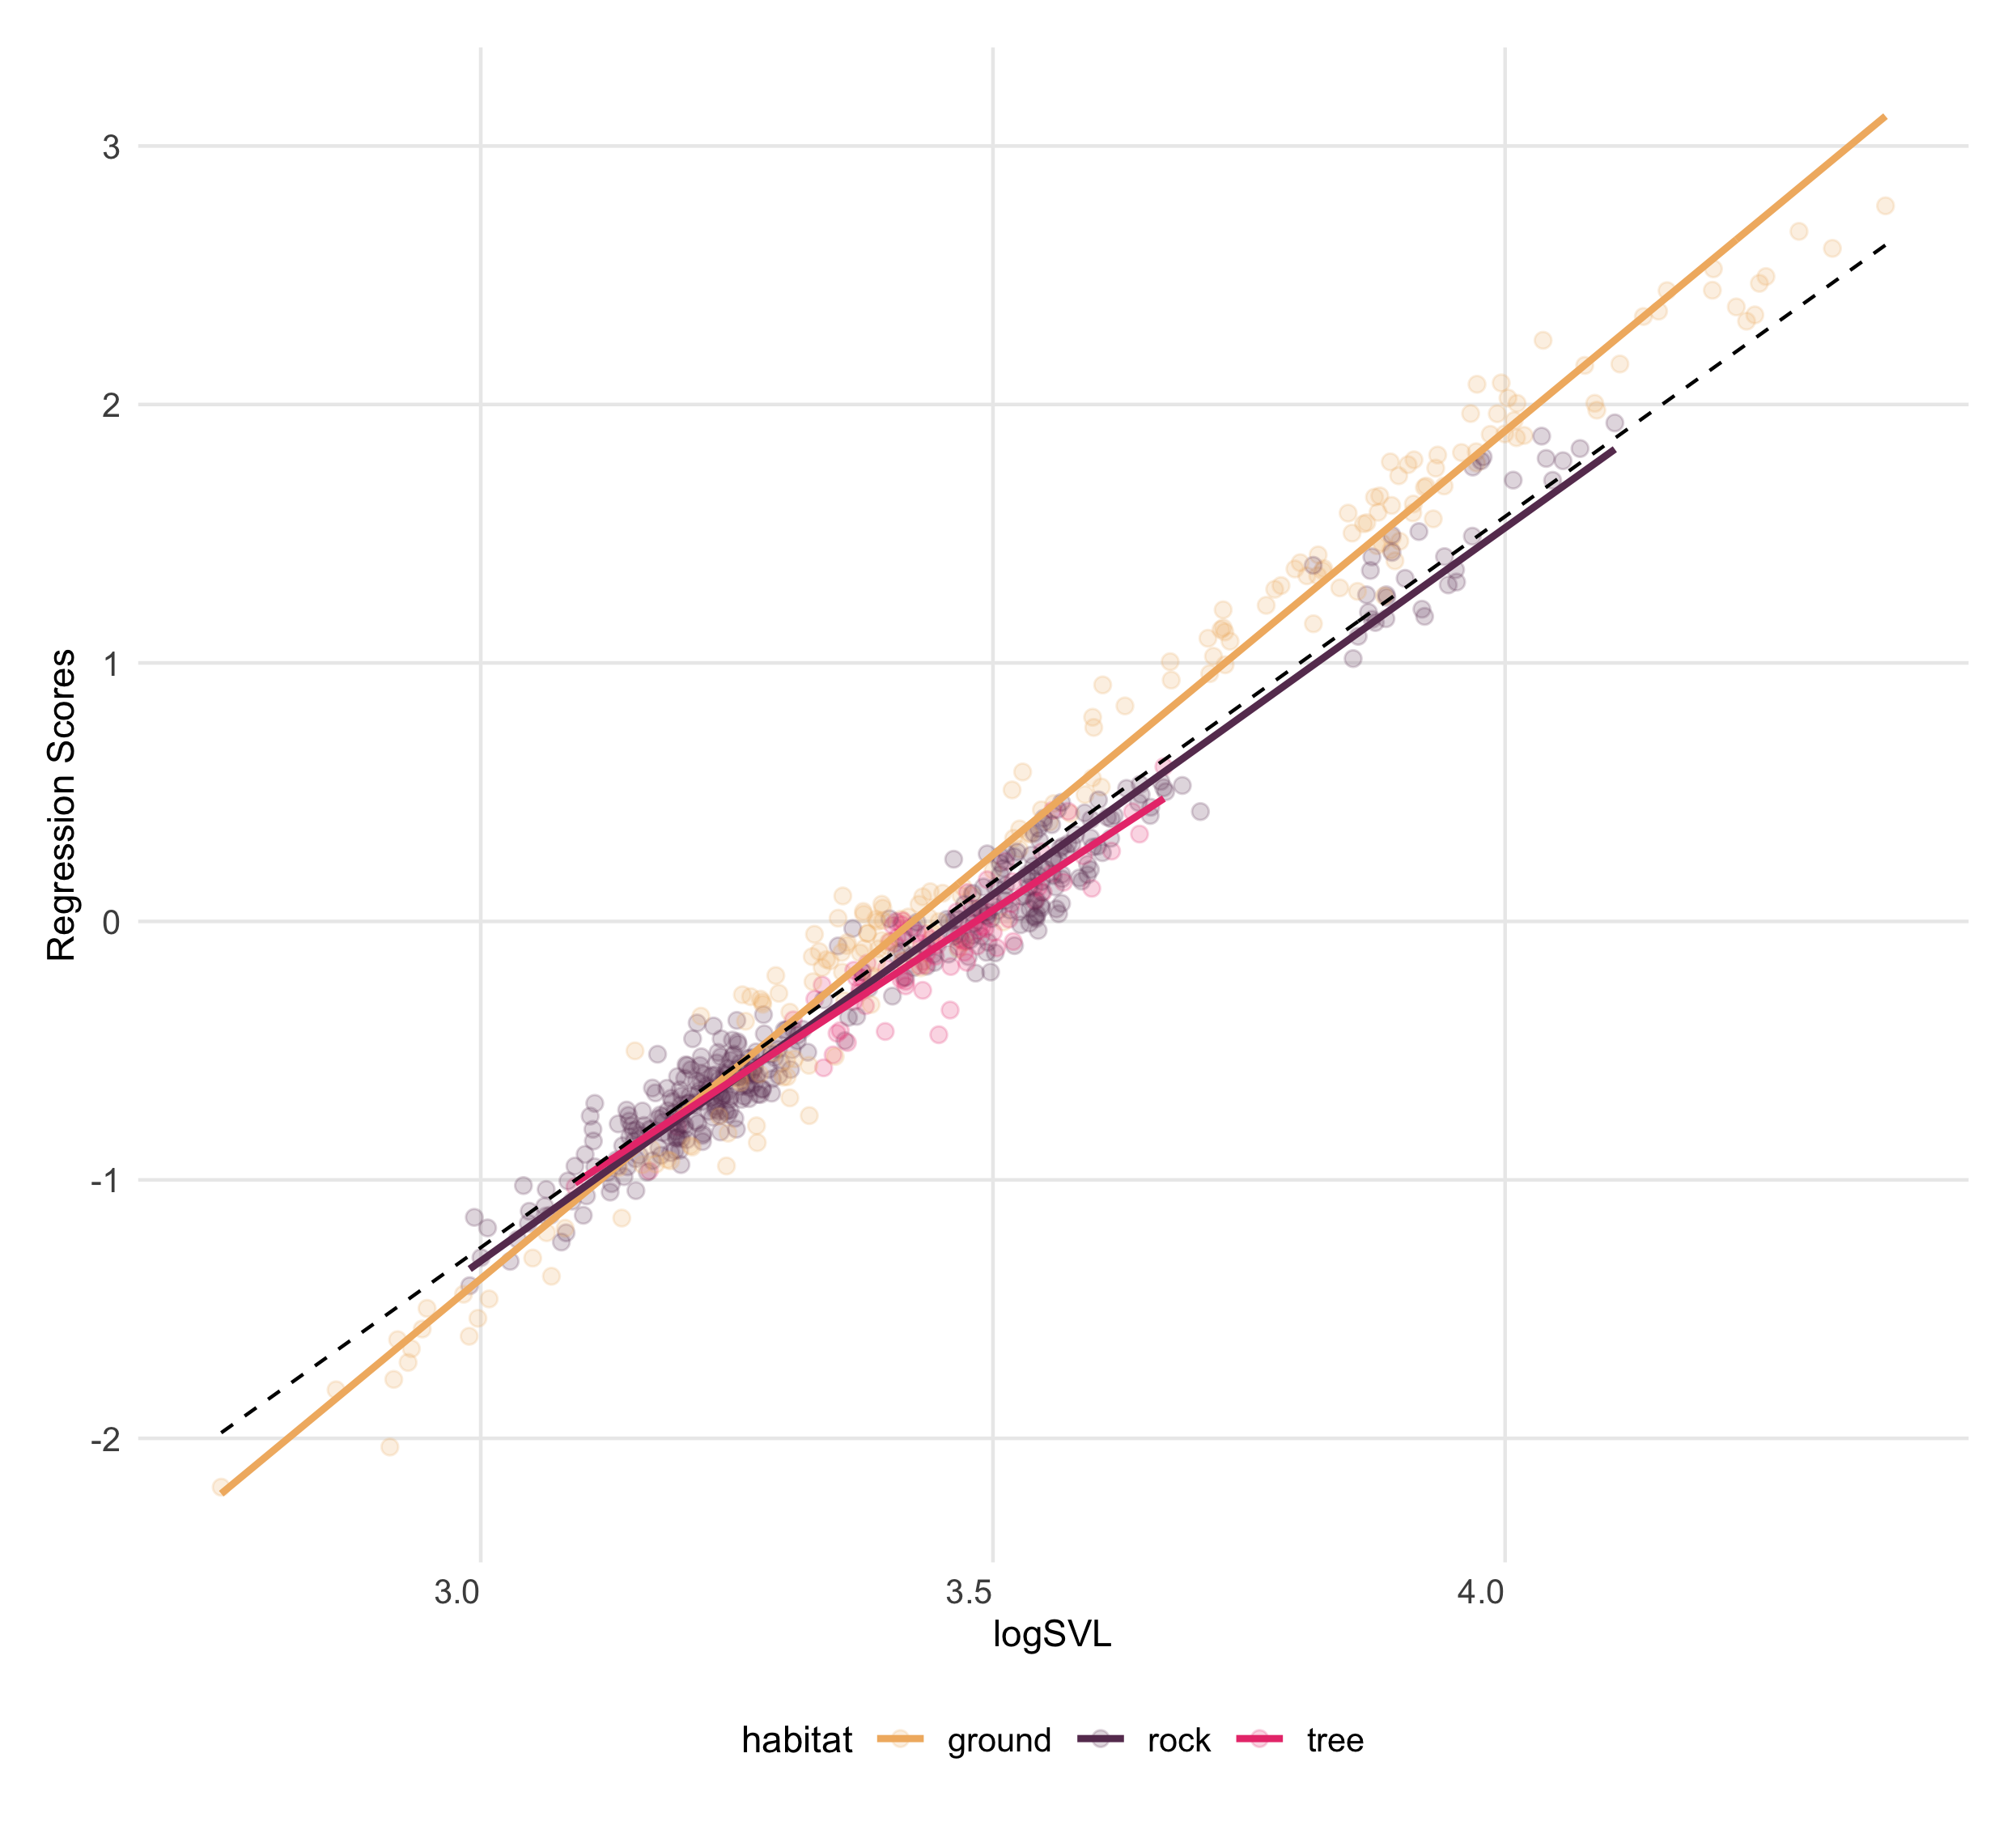
\includegraphics[width=1\linewidth]{Figs/figure_2_ggplot} 

}

\caption{Plot of regression scores and predicted lines representing the relationship between linear body measurements and size (SVL). Individuals are colored by habitat use: ground (beige), rock (dark purple), and tree (magenta). Isometric trend represented by the dashed line.}\label{fig:unnamed-chunk-5}
\end{figure}

\newpage

\begin{figure}

{\centering 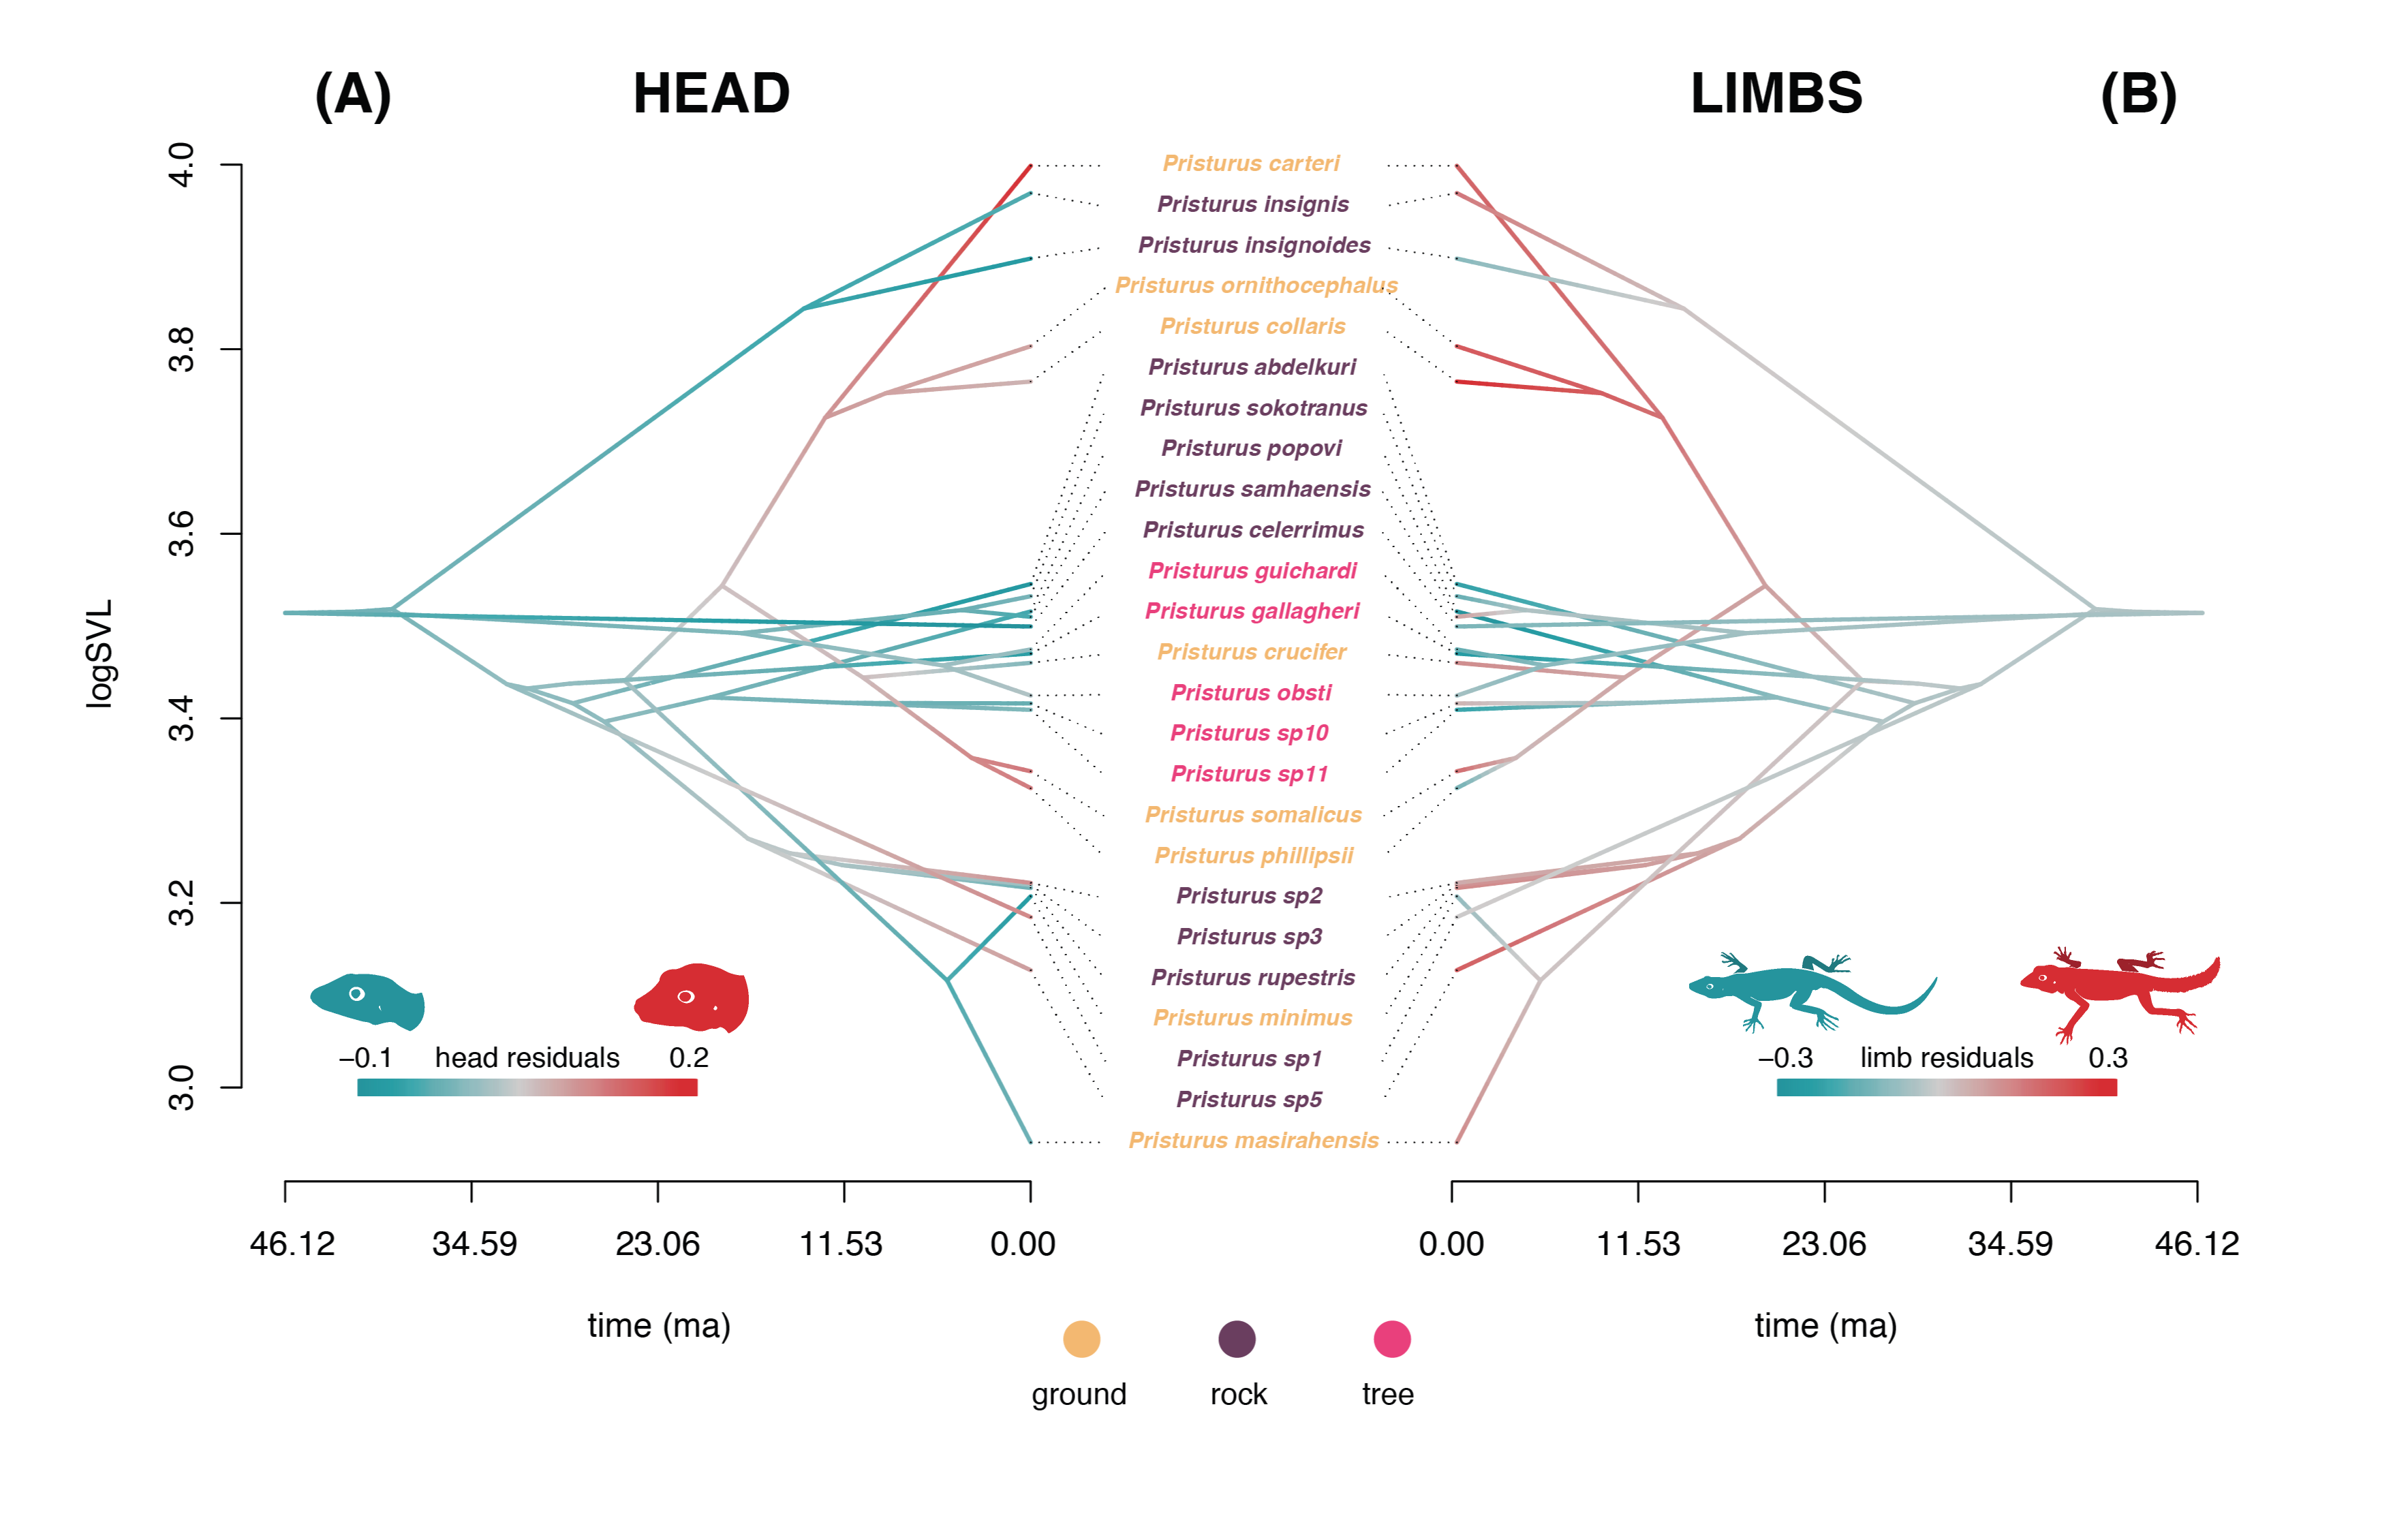
\includegraphics[width=1\linewidth]{Figs/figure_3_Pristurus_allometry_traitgram_legends} 

}

\caption{Traitgrams showing the evolution of body size (SVL) through time based on the phylogenetic tree of \textit{Pristurus}. Colors represent an evolutionary mapping of residuals from phylogenetic regressions describing the relationship of (A) head morphology versus body size, and (B) limb proportions versus body size (see text for descriptions). Species names are colored by habitat use: ground (beige), rock (dark purple), and tree (magenta).}\label{fig:unnamed-chunk-6}
\end{figure}

\newpage

\begin{figure}

{\centering 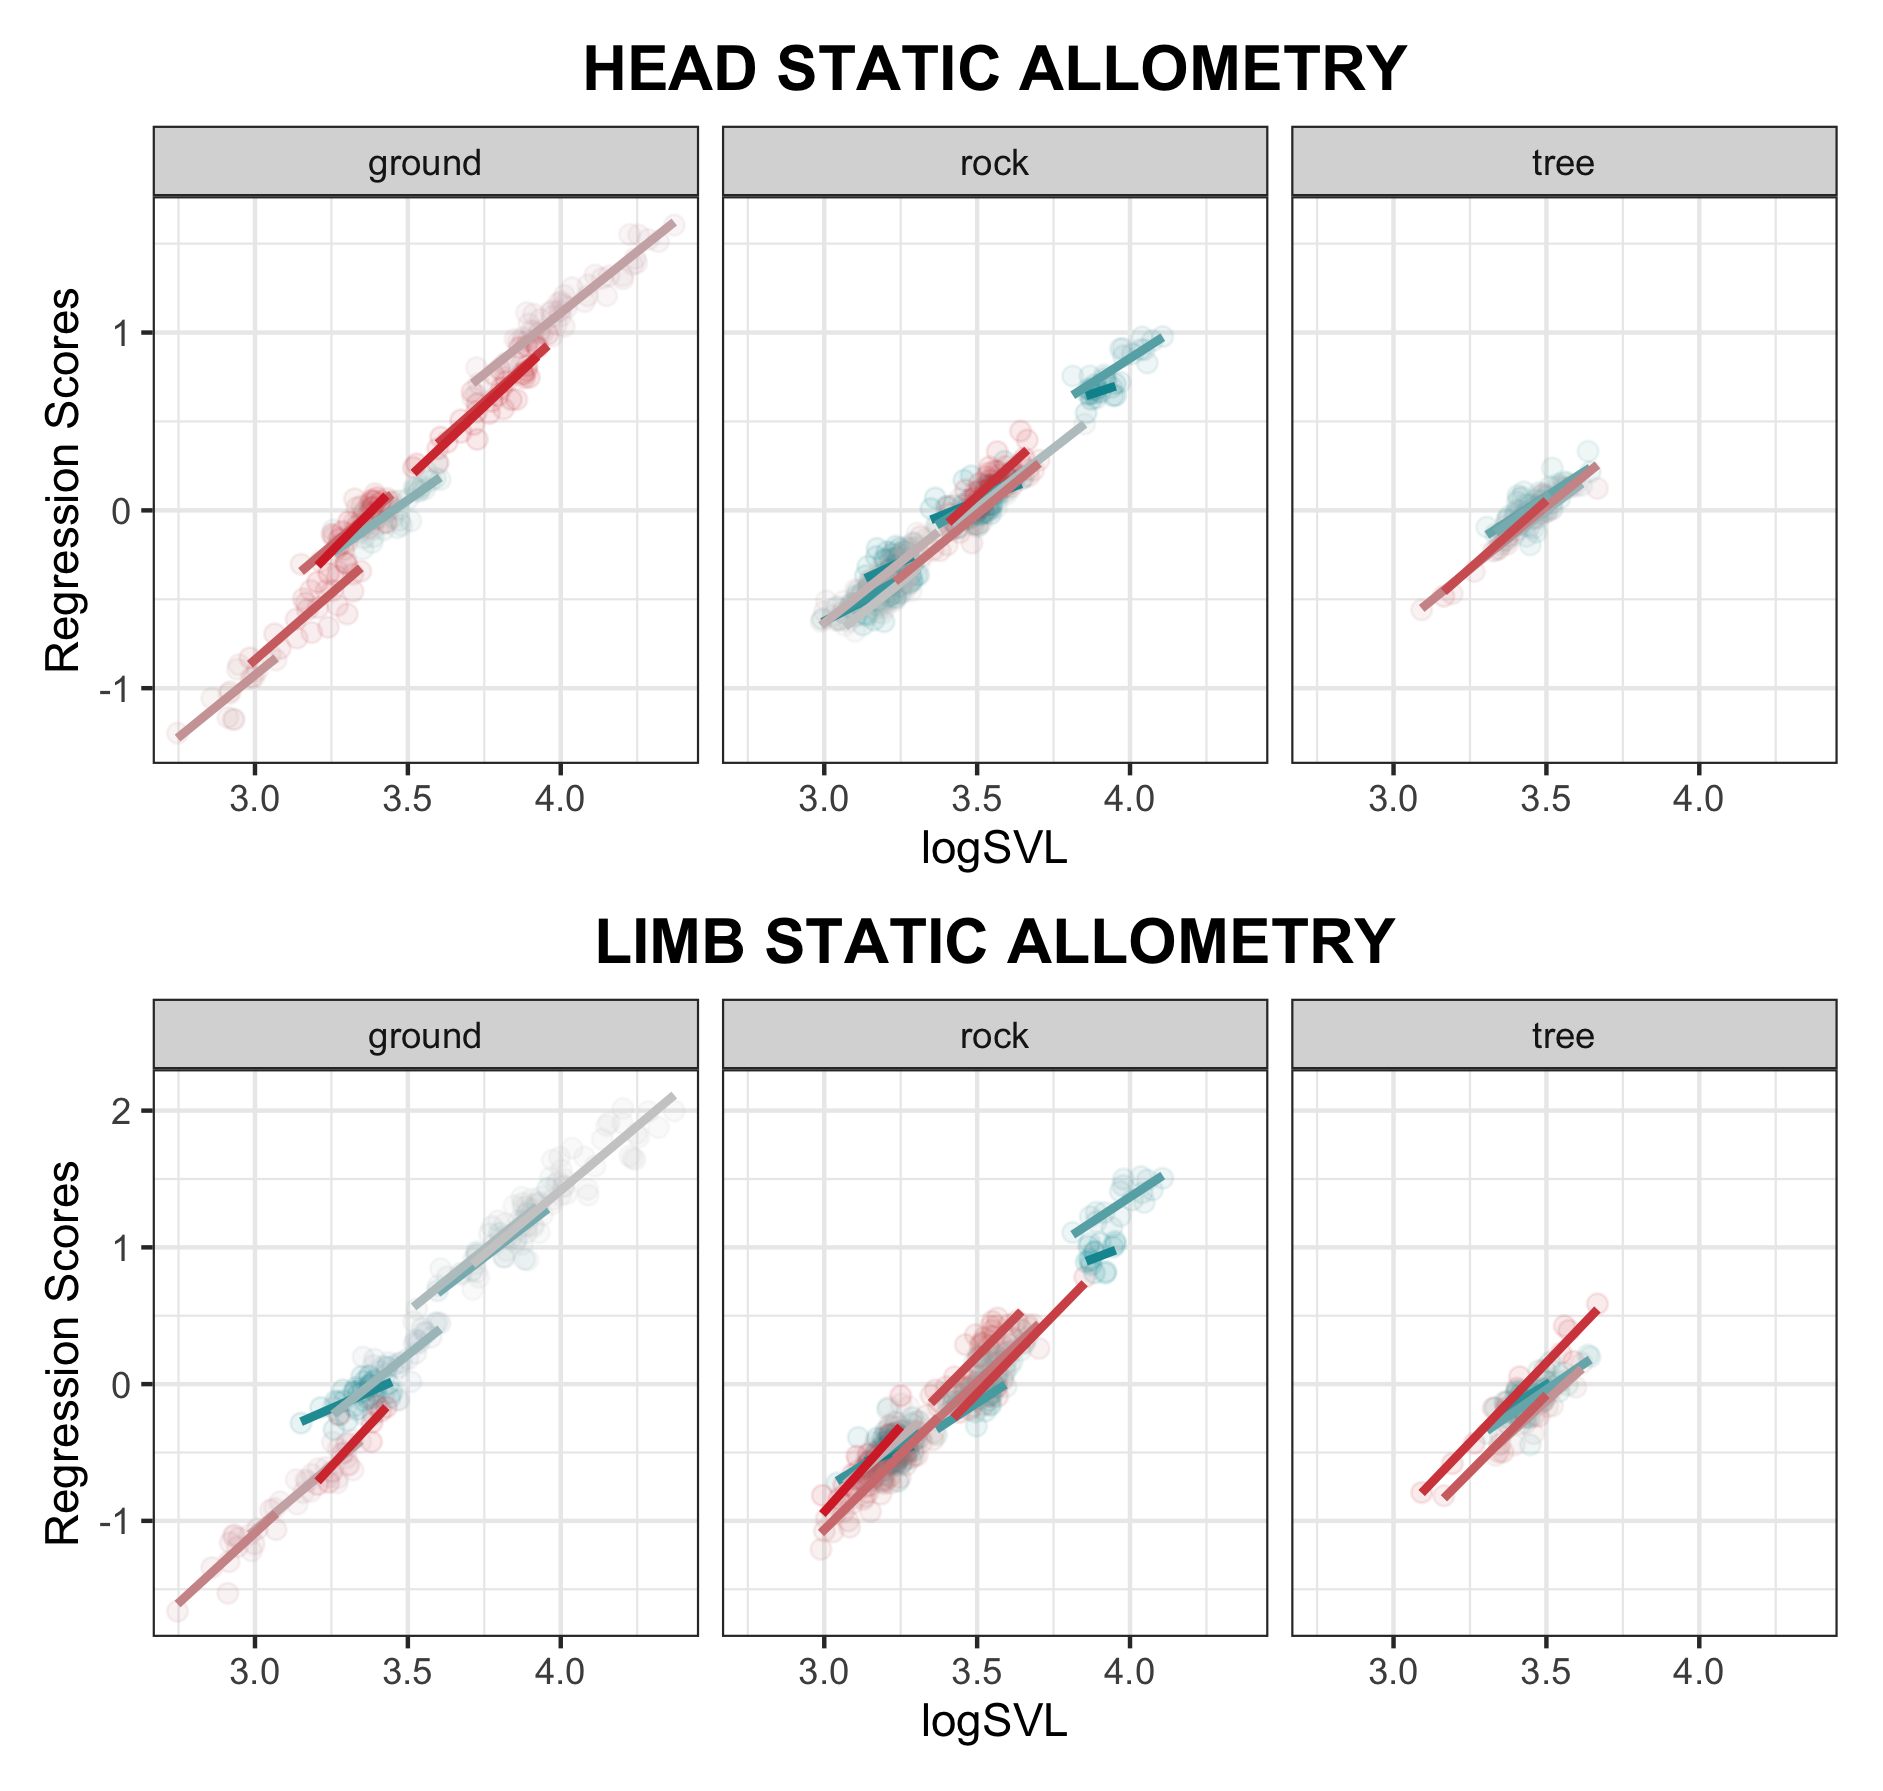
\includegraphics[width=1\linewidth]{Figs/figure_4_static_allometry} 

}

\caption{Patterns of static allometry for each species for head traits (upper panel) and limb traits (lower panel). Species are separated by their habitat groups and colored by the magnitude of their regression slope (red: steeper slopes, blue: shallower slopes).}\label{fig:unnamed-chunk-7}
\end{figure}

\newpage

\begin{figure}

{\centering 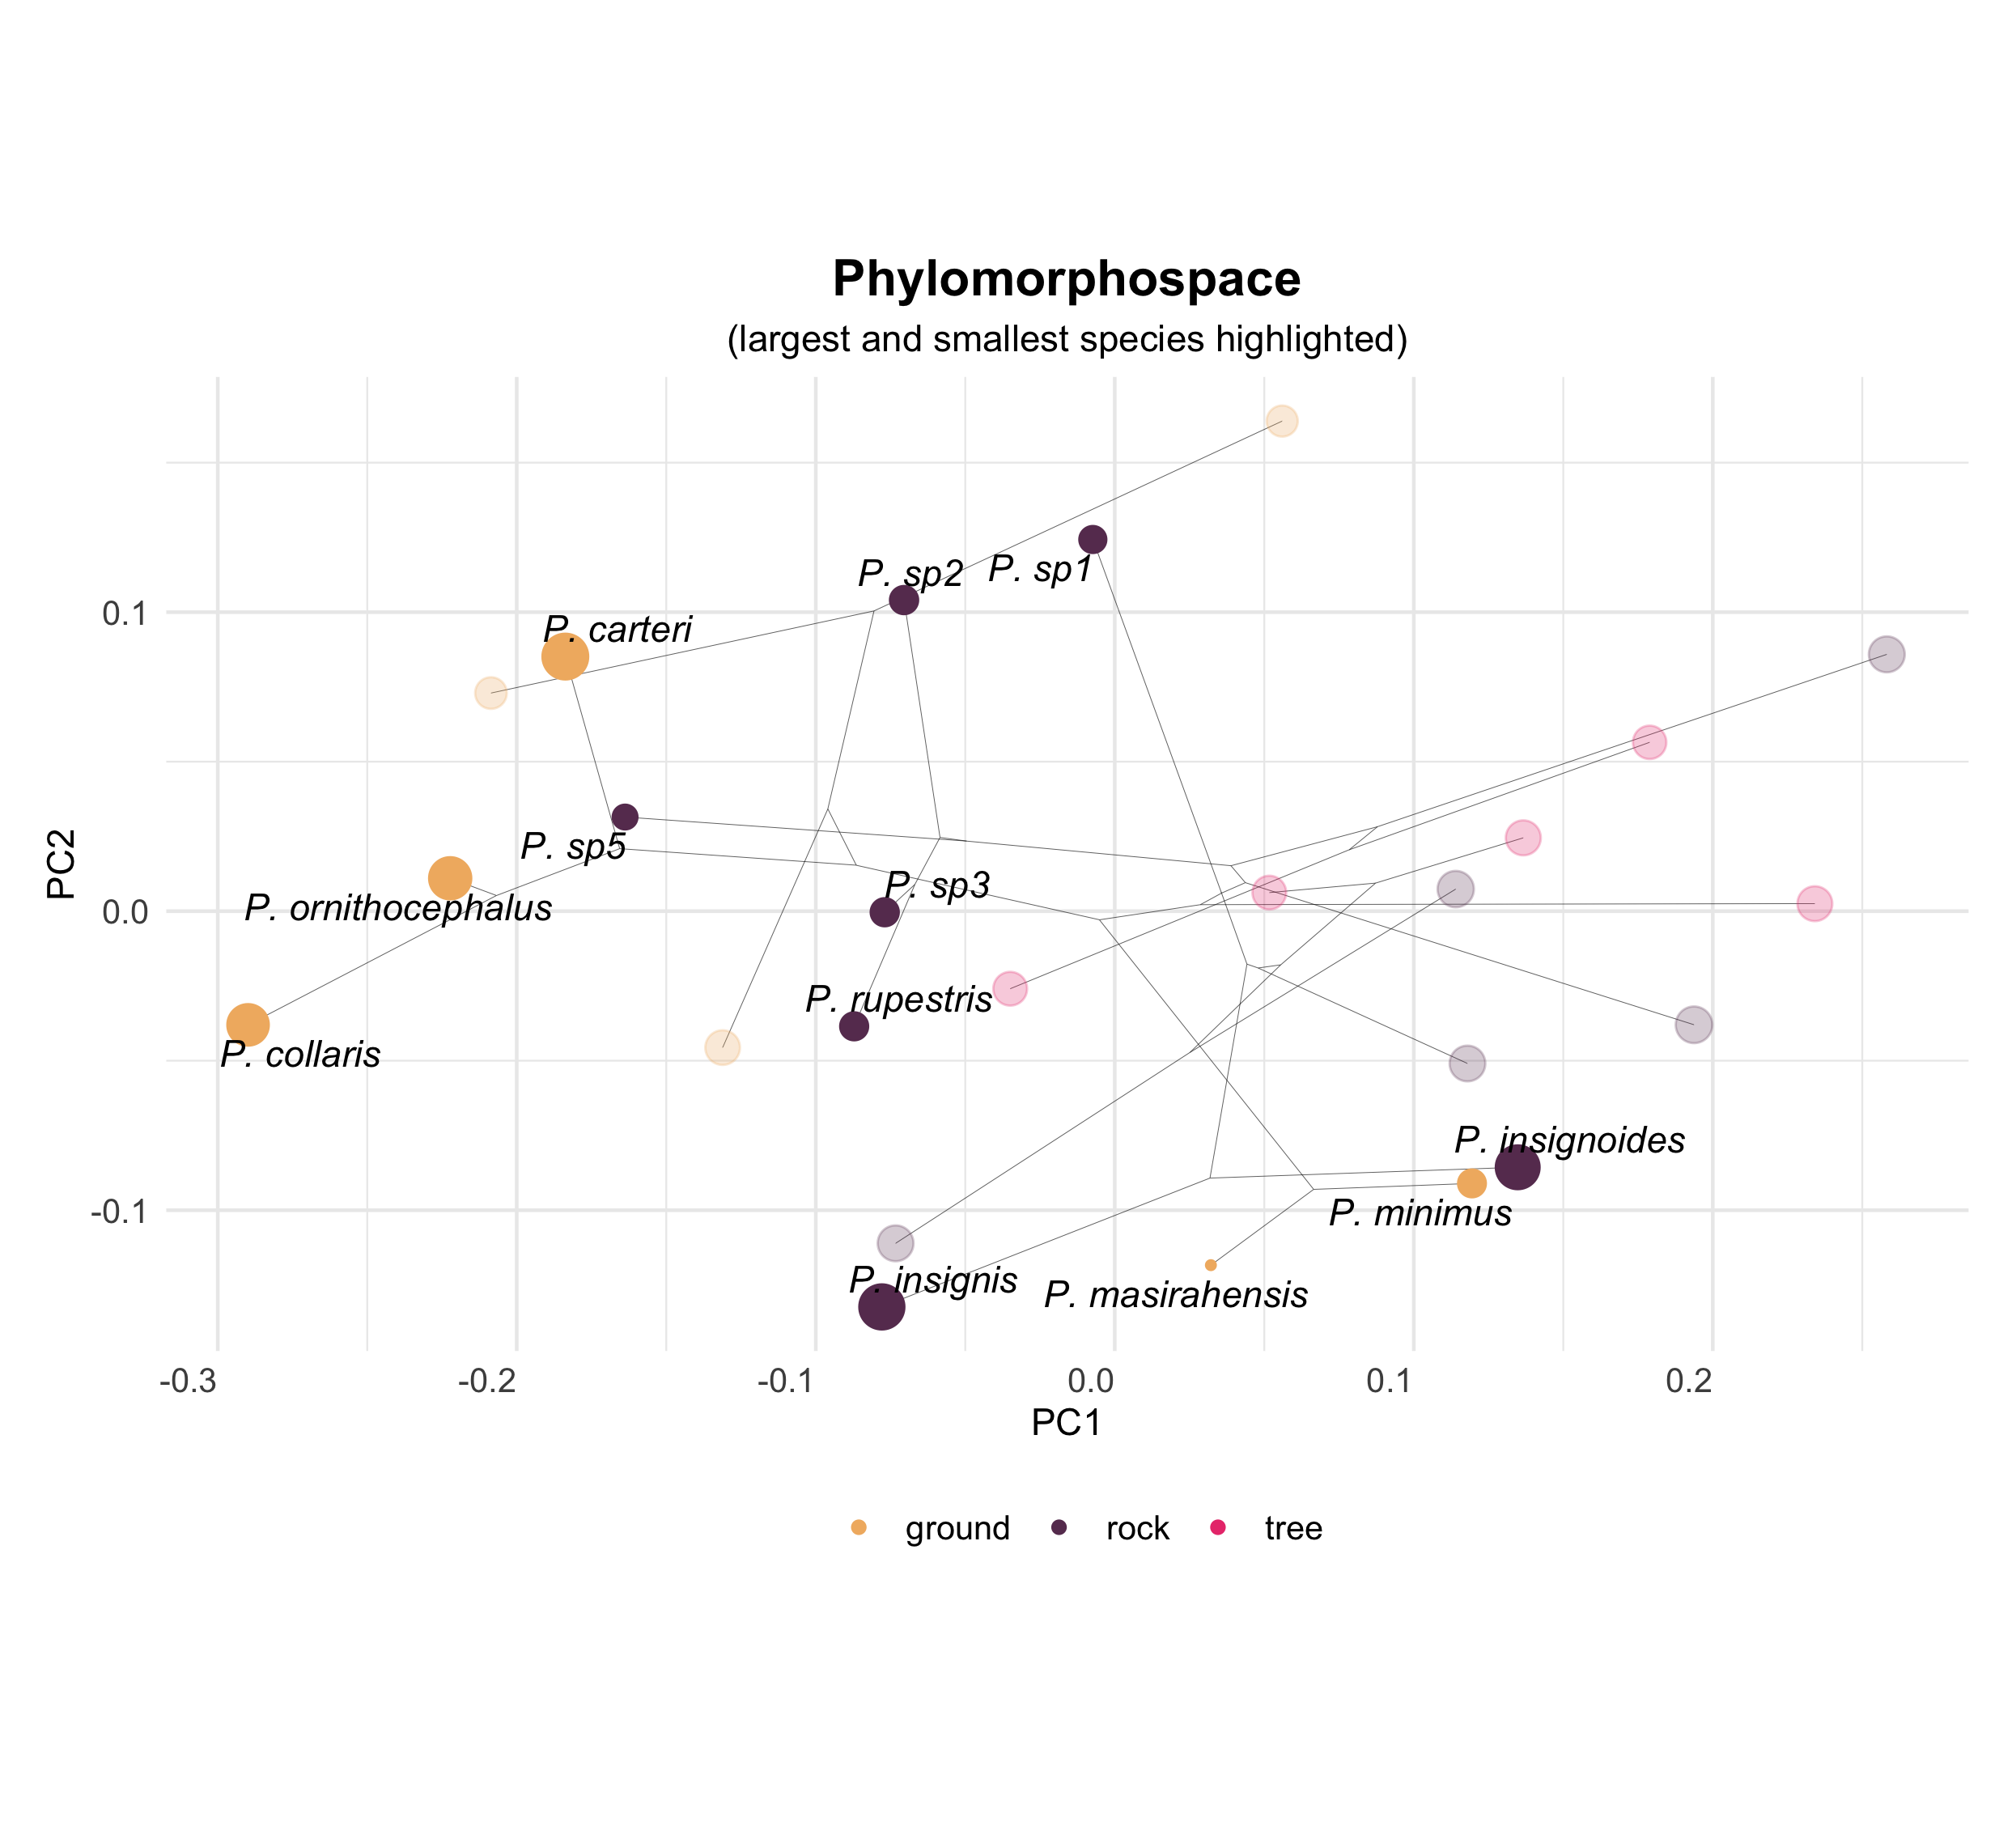
\includegraphics[width=1\linewidth]{Figs/figure_5_phylomorphospace_large_small} 

}

\caption{Phylomorphospace of \textit{Pristurus}, based on residuals from a phylogenetic regression of body measurements on size (SVL). Species means are colored by habitat use: ground (beige), rock (dark purple), and tree (magenta). Large and small rock-dwelling and ground-dwelling are highlighted with darker colors to highlight their differentiation and relative positions in morphospace.}\label{fig:unnamed-chunk-8}
\end{figure}

\newpage

\begin{figure}

{\centering \includegraphics[width=1\linewidth]{Figs/figure_6_Pristurus_allometry_rescaledSVL_horizontal} 

}

\caption{Representative specimens from large and small \textit{Pristurus} species, colored by habitat use: ground (beige) and rock (dark purple). Specimens are scaled to a common body size (SVL) to emphasize the relative differences in limb and head proportions. Original scale shown as the gray bar.}\label{fig:unnamed-chunk-9}
\end{figure}

\end{document}
